\subsection{OCP (Open Catalyst Project)}
{{\footnotesize
\noindent The Open Catalyst Project (OC20 and OC22) provides DFT-calculated catalyst-adsorbate 
relaxation datasets, challenging ML models to predict energies and forces for 
renewable energy applications.


\begin{description}[labelwidth=4cm, labelsep=1em, leftmargin=4cm, itemsep=0.1em, parsep=0em]
  \item[date:] 2020-10-20
  \item[version:] 1
  \item[last\_updated:] 2020-10-20
  \item[expired:] false
  \item[valid:] yes
  \item[valid\_date:] 2020-10-20
  \item[url:] \href{https://opencatalystproject.org/}{https://opencatalystproject.org/}
  \item[doi:] unknown
  \item[domain:] Chemistry; Materials Science
  \item[focus:] Catalyst adsorption energy prediction
  \item[keywords:]
    - DFT relaxations
    - adsorption energy
    - graph neural networks
  \item[licensing:] OCP Terms of Use
  \item[task\_types:]
    - Energy prediction
    - Force prediction
  \item[ai\_capability\_measured:]
    - Prediction of adsorption energies and forces
  \item[metrics:]
    - MAE (energy)
    - MAE (force)
  \item[models:]
    - CGCNN
    - SchNet
    - DimeNet++
    - GemNet-OC
  \item[ml\_motif:]
    - Chemistry
  \item[type:] Benchmark
  \item[ml\_task:]
    - Supervised Learning
  \item[solutions:] 0
  \item[notes:] Public leaderboards; active community development
  \item[contact.name:] unknown
  \item[contact.email:] unknown
  \item[datasets.links.name:] OCP Dataset
  \item[datasets.links.url:] \href{https://fair-chem.github.io/catalysts/datasets/summary}{https://fair-chem.github.io/catalysts/datasets/summary}
  \item[results.links.name:] OCP Pretrained Models
  \item[results.links.url:] \href{https://fair-chem.github.io/catalysts/models.html}{https://fair-chem.github.io/catalysts/models.html}
  \item[fair.reproducible:] True
  \item[fair.benchmark\_ready:] True
  \item[id:] ocp\_open\_catalyst\_project
  \item[Citations:] \cite{chanussot2021oc20}, \cite{tran2023oc22}, \cite{doi:10.1021/acscatal.0c04525}, \cite{tran2023b}
\end{description}

{\bf Ratings:} ~ \\

\begin{tabular}{p{0.15\textwidth} p{0.07\textwidth} p{0.7\textwidth}}
\hline
Rating & Value & Reason \\
\hline
dataset & 5 & Fully FAIR- OC20, per-adsorbate trajectories, and OC22 are versioned; datasets come with standardized splits, metadata, and are downloadable.
 \\
documentation & 1 & Paper exists, but content is behind a paywall.
 \\
metrics & 5 & MAE (energy and force) are standard and reproducible.
 \\
reference\_solution & 4 & Multiple baselines (GemNet-OC, DimeNet++, etc.) implemented and evaluated. No hardware listed.
 \\
software & 5 & Data provided in Github links
 \\
specification & 5 & Tasks (energy and force prediction) are clearly defined with explicit I/O specifications, constraints, and physical relevance for renewable energy.
 \\
\hline
\end{tabular}

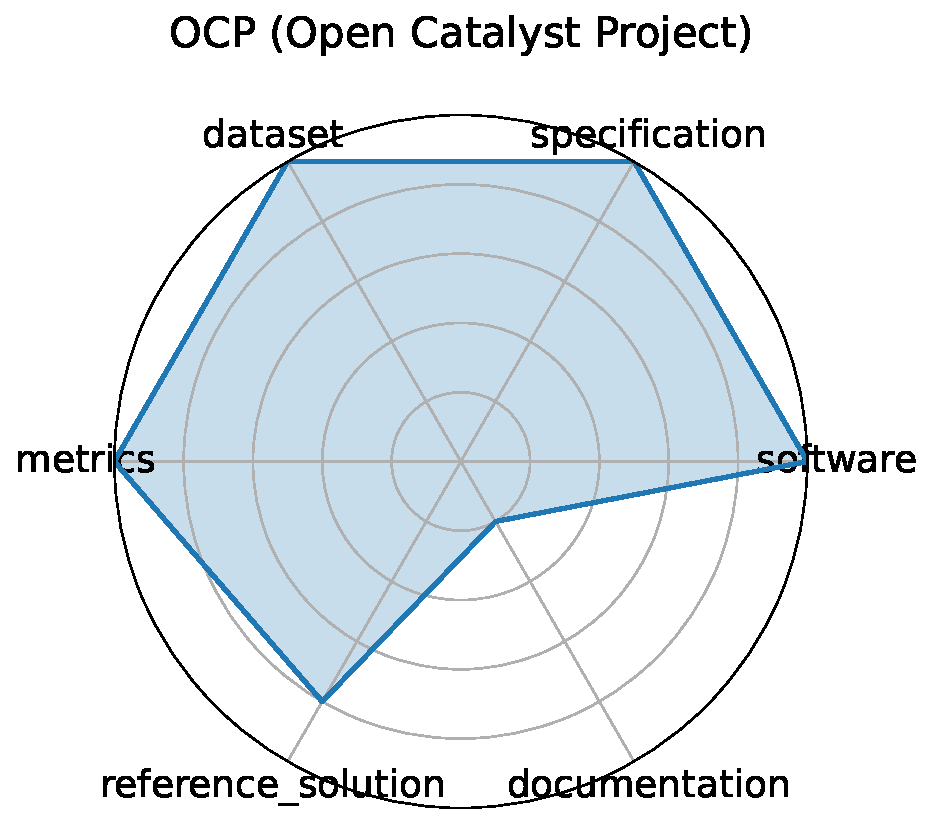
\includegraphics[width=0.2\textwidth]{ocp_open_catalyst_project_radar.pdf}
}}
\clearpage